\documentclass[12pt,letterpaper]{article}
\usepackage[margin=1.0in]{geometry}
\usepackage[utf8]{inputenc}
\usepackage{cite}
\usepackage{amsmath}
\usepackage{amsfonts}
\usepackage{amssymb}
\usepackage{makeidx}
\usepackage{graphicx}
\usepackage{hyperref}
\setlength\parindent{0pt}
\usepackage[framed,numbered,autolinebreaks,useliterate]{mcode}

\author{NAME:}
\title{HW: Controller Area Network (CAN) data analysis.}

\begin{document}

\maketitle

\section{Objectives}
The objective of this homework is to familiarize students with CAN data and analyze them using Excel, MatLab and Google Earth. 

\section{Introduction}
Modern vehicles including cars, trucks/buses as well as off-road equipment have a computer network that serves to manage the drive train, interaction with the operator, as well as to communicate with implements. We can tap into this computer network and record a host of messages that contain data that we are interested in during operations.\\

The data we are going to analyze were collected during a tillage operation with a John Deere tractor in spring 2016 using a Vector CAN data interface. The Vector unit was programmed to record data such as GPS location, Engine torque, RPM, as well as Wheel Speed, Ground Speed and Fuel consumption. Vector provides a tool that allow us to translate the proprietary Vector (xlx) format into an Excel readable format. The identifier and the data are in hexadecimal format, so we need to convert them to decimal format to extract the GPS coordinates in Latitude/ Longitude form. The Excel file that contains our data has the filename 60519009.xls. We are going to open this file in Excel, convert the strings into cells using Excel's text to column function, then we are going to extract only GPS data, we will convert them to decimal format, and copy and paste all our coordinates into a text file (either using Notepad or MatLab's editor). We will then use a small MatLab program that translates these coordinates into a kml file. This file will be read by Google Earth which will show our GPS locations graphically.\\

\section{Procedures}

The standard CAN message that shows the GPS location of a vehicle, is as follows: Note that the identifier is given in hexadecimal format. You can always convert the hexadecimal number into a decimal number, but the hexadecimal notation is far more compact and elegant. As you can see from the definition, the GPS location has the identifier CFEF31C, and it contains 8 bytes (that is 64 bits). The first 4 bytes represent the Longitude and the second 4 bytes the Latitude. After we convert the Lat and Lon data to decimal, we need to multiply that decimal number by a scaling factor of $10^{-7}$ and add an offset of -210. Since this field is in central Illinois, the latitude always starts with 40 and the longitude with -88 (going west from Greenwich in the UK yields a negative number).

\begin{itemize}
	\item   CFEF31C – Vehicle Position
	\item	Latitude
	\subitem	Bit Start: 0
	\subitem	Bits: 32
	\subitem	Scaling Factor: .0000001
	\subitem	Offset: -210
	\item	Longitude
	\subitem	Bit Start: 32
	\subitem	Bits: 32
	\subitem	Scaling Factor: .0000001
	\subitem	Offset: -210
\end{itemize}
\begin{enumerate}
	\item First open the CAN data file 60519009.xls in Excel format (answer yes on the question whether you want to open it).
	
	Select column A and now perform a text to column operation using tab, space and the colon (special character as delimiters), see Figure \ref{fig:TextToColumnDelimiters}. Be patient, for a large datafile like this it will take a while to do this.
	
	\begin{figure}
		\centering
		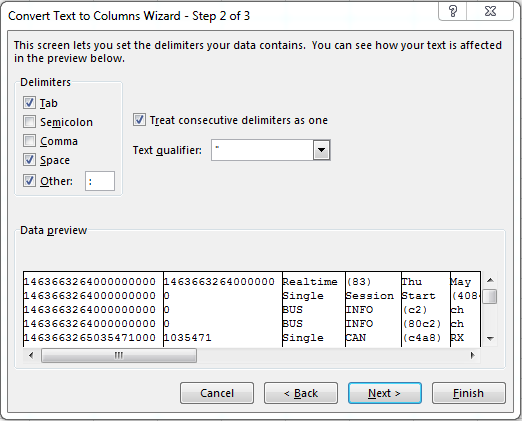
\includegraphics[width=0.8\linewidth]{TextToColumnDelimiters}
		\caption{Text To Column Delimiters choice in Excel}
		\label{fig:TextToColumnDelimiters}
	\end{figure}
	
	If you did it right now column L should contain the CAN message identifiers. Now you want to sort everything on column L so we can select only messages that contain GPS data, which have the identifier CFEF31C. MAKE SURE to select ALL columns before you sort on column L, otherwise the GPS data and the identifier are no longer matched. 
	\item Remove all records (rows) that do not have the identifier CFEF31C. If all went well you should have 14,261 records.
	
	\item 	Save your file as "CANDataAnalysis\_YourName.xlsx" in excel format (not text).
	\item	Now we are going to extract the data from the GPS records. The standard says that the Latitude is contained in bytes 1-4 (that is 32 bits) of the datastring, and that the Longitude is contained in bytes 5-8. If you look in the datafile you will see not only numbers but also letters. This is because the data is given in the hexadecimal format so we need to first convert it into decimal format. We do this in a couple of steps: Firstly, we will convert all hexadecimal data into decimal data using Excel's hex2dec function. Start with the first record and in column W type =hex2dec(N1) copy this over to all 7 cells to the right of it.\\
	
	Now we need to calculate the Latitude and the Longitude from the decimal data records. The basis of our decimal data is 256. Therefore the Latitude will be (assuming the data is in columns W-AD, see Figure \ref{fig:FinalExcelSpreadsheet}):\\
	
	Cell AE\\
	
	$=(AD1+AC1*256+AB1*256^2+AA1*256^3)*0.0000001-210$
	
	The factor $10^{-7}$ is the scaling factor and the -210 is the offset, see the definition of the Vehicle position in the standard. 
	
	Do the same thing for Cell AF:\\
	
	$=(Z1+Y1*256+X1*256^2+W1*256^3)*0.0000001-210$	
	
	Copy cells W1 through AF1 over all the way to the last record in the file. Now you should have two columns one for the Latitude column AE () and one for the Longitude (column AF) containing 14,261 GPS coordinates. ALL GPS coordinates should start with 40 for the latitude and -88 for the longitude records.
	
	\begin{figure}
		\centering
		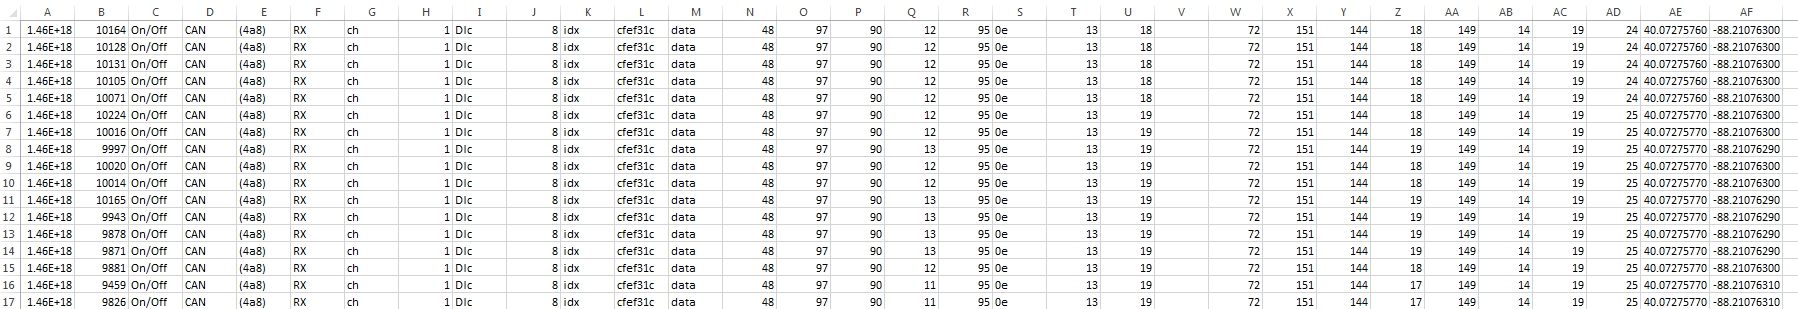
\includegraphics[width=1\linewidth]{FinalExcelSpreadsheet}
		\caption{This is what your spreadsheet should look like when you are done with it.}
		\label{fig:FinalExcelSpreadsheet}
	\end{figure}

	\item Copy ALL GPS coordinates (that is two columns and 14,261 rows), start Matlab, and open its editor (type edit). Now paste these two columns into a new file and save that file as GPSdataDemo.txt, \textbf{make sure you save it as a text file, not a m-file}. 
	\item Type in (or copy from the tex file) the code shown below. Save this file as CANDataAnalysis.m (with extension m, since it is an executable MatLab script, make sure it is saved in the same folder where your GPSdataDemo.txt file resides). The program will load your GPSdataDemo.txt file and write the GPS coordinates in kml format which Google Earth can read.
	\begin{lstlisting}
	close all
	clear all
	clc
	
	KML_filename = 'GPSdataDemo.kml';
	load GPSdataDemo.txt;
	
	FieldPlots   = struct('lat', GPSdataDemo(:,1), 'lon', GPSdataDemo(:,2));
	
	kmlwritepoint([KML_filename], FieldPlots.lat, FieldPlots.lon);
	\end{lstlisting}
	
	\item Find your kml file and double click on it. This will open Google Earth, and if all went well, show the exact coordinates where the machine traveled. If MatLab throws an error in the kmlwritepoint line, that means that the Mapping toolbox is not installed, in that case finish this homework in the computer lab (220).

\end{enumerate}

\section{Submission}

Add a screenshot of the output that you saw in Google Earth to this file. Given in the tex file is the code to add a figure commented out, save the screenshot as AgEngineeringFarmGPS\_GoogleEarth.png.

%	\begin{figure}
%		\centering
%		\includegraphics[width=1\linewidth]{AgEngineeringFarmGPS_GoogleEarth}
%		\caption{Google Earth output screen shot.}
%		\label{fig:AgEngineeringFarmGPS_GoogleEarth.PNG}
%	\end{figure}

\end{document}
